\chapter{Complex Analysis}

\section{Complex Numbers $\mathbb C$}
\subsection{Imaginary unit}
We define $i$ to be the imaginary unit, such that $i^2=-1$. Any complex number can be decomposed into two parts:
$$
z=x+yi\qquad x,y\in\mathbb R
$$
where $x=\operatorname{Re}(z)$ and $y=\operatorname{Im}(z)$.

We can see many similarities of $\mathbb C$ and $\mathbb R^2$.

\subsection{Complex Conjugate}
We define the Complex conjugate $\overline z$ as: 
$$
\overline z = x-yi
$$
\begin{figure}[H]
    \begin{center}
    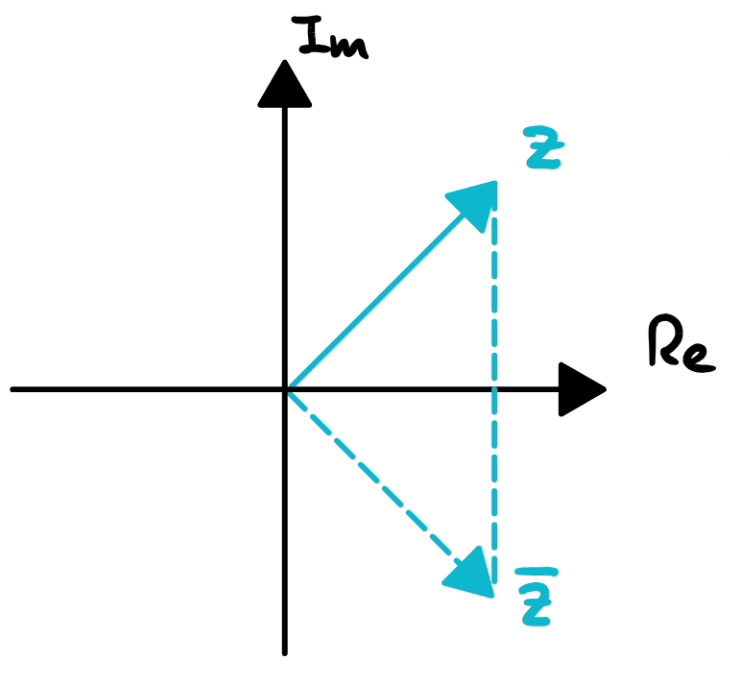
\includegraphics[width=0.4\textwidth]{ComplexConjugate.png}
    \caption{plot real and imaginary part with complex conjugate as vectors}
    \end{center}
\end{figure}

\subsection{Modulus (Absolute Value)}
We define the modulus to be
$$
\lvert z \rvert = \sqrt{x^2+y^2}
$$
If $z_0,z_1\in\mathbb C$, then the distance between the two points can be described by $\lvert z_1-z_0\rvert$.


\subsection{Euler's Formula}
For $\theta\in \mathbb R$: 
$$
e^{i\theta} = \cos\theta + i\sin\theta
$$

\begin{figure}[H]
    \begin{center}
    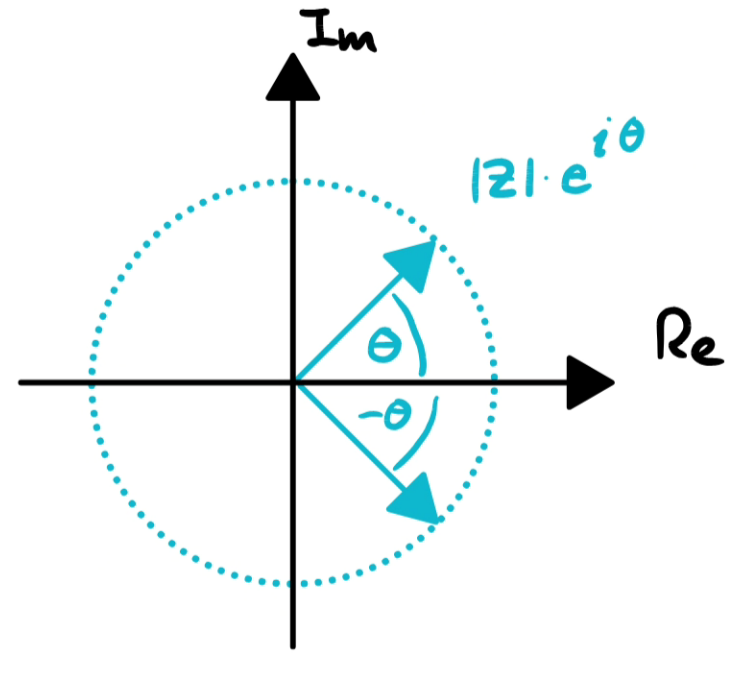
\includegraphics[width=0.4\textwidth]{PolarExpression.png}
    \caption{plot with circle showcasing $e^{i\theta}$, similar to polar coordinates}
    \end{center}
\end{figure}

 
This yields the observations:
\begin{itemize}
    \item $\lvert e^{i\theta}\rvert = 1$
    \item $\overline{\lvert e^{i\theta}\rvert} = \rvert e^{-i\theta}\rvert$
\end{itemize}

\subsubsection{Algebraic Operations}
with two imaginary numbers $z_1=x_1+iy_1, z_2=x_2+iy2$ the basic operations are as follows:
\begin{itemize}
    \item {Addition} $z_1\pm z_2 = (x_1\pm x_2) + i(y_1\pm y_2)$
    \item {Multiplication} $z_1\cdot  z_2 = (x_1 + iy_1) \cdot  (x_2+i y_2) = (x_1x_2-y_1y_2)+i(x_1y_2+x_2y_1)$
    \item {Multiplication with complex conjugate} $z\cdot \overline z = \lvert z\rvert ^2$
\end{itemize}
Note that multiplication with the complex conjugate can be useful for expanding fractions: 
$$
\frac{z_1}{z_2}=\frac{z_1\overline{z_2}}{\lvert z_2\rvert ^2}
$$

\subsection{Polar expression}
For complex numbers $z_n=\lvert z\rvert \cdot e^{i\theta}$ to be the same, we need:

\begin{equation*}
z_1=z_2
\Rightarrow 
\begin{cases}
|z_1|=|z_2|\\
\theta_1-\theta_2 \in 2\pi \mathbb Z
\end{cases}
\end{equation*}
\subsubsection{Principal Argument}
The argument can be thought of as the angle between the horizontal line and $z$ as a vector around the origin in counter clockwise direction.
$$
\operatorname{Arg}(z)\in]-\pi,+\pi]\implies z= |z| \cdot e^{i\operatorname{Arg}(z)}
$$
$$
\operatorname{Arg}(z) = \begin{cases}
	\arctan y/x&x > 0\\
	\pi/2&x=0,y>0\\
	\pi + \arctan y/x&x<0,y\ge0\\
	-\pi/2&x=0,y<0\\
	-\pi+ \arctan y/x&x<0,y<0
\end{cases}
$$


\subsubsection{Algebraic Operations}
With the polar expression multiplication of two complex numbers yields:
\begin{equation*}
\begin{split}
    z_1\cdot z_2 &= |z_1||z_2|e^{i(\theta_1+\theta_2)}\\
    \frac{z_1}{z_2} &= \frac{|z_1|}{|z_2|}e^{i(\theta_1-\theta_2)} 
\end{split}
\end{equation*}

We can conclude that if $x=0, \theta =\pm\pi/2$ and if $x\ne 0, \theta = \arctan\frac yx$.

\subsection{Examples}
To solve $z^5=2$ for $z$, we use the polar expression:
\begin{equation*}
\begin{split}
|z|^5 \cdot e^{i5\operatorname{Arg}(z)}=2&=2\cdot e^{i0}\\
&\implies
\begin{cases}
    \operatorname{Arg}(z) \in \frac 25\pi \mathbb Z\\
    \operatorname{Arg}(z) \in]-\pi,\pi]
\end{cases}\\
&\implies
\operatorname{Arg}(z)\in\left\{-\frac{4\pi}5,-\frac{2\pi}5 , 0, \frac{2\pi}5, \frac{4\pi}{5}\right\}
\end{split}
\end{equation*}

\section{Complex Functions}
A complex function $f: \mathbb C \to\mathbb C$ is a function that takes a complex variable and returns another complex number that can be decomposed into a real and imaginary parts. We can therefore think of them as two functions, $u, v: \mathbb R^2 \to \mathbb R$:
\begin{equation*}
\begin{split}
z:x+iy\to f(z)=u(x,y)+i\cdot v(x,y)
\end{split}
\end{equation*}

\subsection{Important Complex Functions}
\begin{itemize}
    \item $f(z)=z=x+yi$
    \item $f(z)=\overline z=x-yi$
    \item $f(z)=z^2=x^2-y^2+2xyi$
    \item $f(z)=e^z=e^{x+iy}=e^x=e^x(\cos y+i\sin y)=e^x\cos y + i(e^x\sin y)$
    \item $\cos(z)=\frac{e^{iz}+e^{-iz}}2$
    \item $\sin(z)=\frac{e^{iz}-e^{-iz}}2$
    \item $\cosh(z)=\frac{e^z+e^-i}{2}$
    \item $\sinh(z)=\frac{e^z-e^-i}{2}$
\end{itemize}
\textbf{Note:} The complex exponent function $\exp$ here is assumed to behave exactly as it would with real functions.

As an example, we can try to find the real and imaginary parts of the cosine function:
\begin{equation*}
\begin{split}
\cos(z)&=\cos(x+yi)\\
&=\frac{e^{i(x+yi)}+e^{-i(x+yi)}}2\\
&=\frac 12 \left(e^{-y}e^{ix}+e^ye^{-ix}\right)\\
&=\frac 12(e^{-y}+e^y)\cos x + \frac i2 (e^y-e^y)\sin x\\
&=\cosh y\cdot \cos x + i \sinh y \sin x
\end{split}
\end{equation*}
Which is an important identity.

\subsection{Definition: Limits and continuity}
We will say that $z_n\stackrel{n}{\rightarrow}z_0$ 
if for any $\varepsilon > 0$, there exists $N > 0$ such that  for any $n > N$, $|z_n-z_0| < \varepsilon$, $\lim_{n\to +\infty} z_n = z_0$.

Let $f:\mathbb C \to \mathbb C$ and $z_0\in \mathbb C$. We will say that $f$ is continuous at $z_0$ if for any $\varepsilon > 0 $, there exists a $\delta > 0$ such that when $|z-z_0| < \delta\implies |f(z)-f(z_0)| < \varepsilon$.
Equivalently, $\lim_{z\to z_0} = f(z_0)$.

Let $f(x+yi) = u(x,y)+iv(x,y)$. $f$ is continuous at $z_0=x_0+y_0i\Leftrightarrow$ $u$ and $v$ are continuous at $(x_0,y_0)$.

$f$ is continuous at a point $z_0\Leftrightarrow$ for every sequence $z_n\stackrel{n\to\infty}\to z_0$ the images converge: $f(z_n)\stackrel{n\to\infty}\to f(z_0)$ 

\subsection{Differentiability, Holomorphic and Entire Functions}
Let $f:\mathbb C \to\mathbb C$ be a complex function. We will say that $f$ is (complex) differentiable at $z_0$ if the limit $$\lim_{z\to z_0} \frac{f(z)-f(z_0)}{z-z_0}$$ exists, is finite, and is denoted by $f'(z_0)$.

\begin{itemize}
    \item if $f$ is differentiable at every point of an open set $W$ then $f$ is \textbf{holomorphic} on $W$.
    \item if $f$ is holomorphic on $\mathbb C$ then $f$ is \textbf{entire}.
\end{itemize}
\textbf{Reminder:} A set $W\subseteq \mathbb C$ is open if $\forall z_0 \in W\exists \varepsilon > 0$ such that $D=\{z:|z-z_0|<\varepsilon\}\subseteq W$.

\subsubsection{Examples}
To differentiate $f(z)=z$ at $z_0$ we take the limit:
$$
f'(z_0) = \lim_{z\to z_0} \frac{z-z_0}{z-z_0} = 1
$$
When differentiating $f(z)=1/z$ on $\mathbb C^\ast$ we get that $$f'(z)=-\frac 1{z^2}$$ Which shows that $f$ is holomorphic on $\mathbb C^\ast$.

\subsubsection{Properties}
\begin{itemize}
    \item If $f$,$g$ are continuous / differentiable at $z_0$ then the same is true for $f+g$ and $f\cdot g$.
    \item Derivative of a product and of compositions are the same as on $\mathbb{R}$.
\end{itemize}

\subsection{Cauchy-Riemann Equations}
\paragraph{Recall} A function $f:\mathbb C \to \mathbb C$ is complex differentiable at $z_0\in\mathbb C$ if the limit $$f'(z_0)=\lim_{z\to z_0} \frac{f(z)-f(z_0)}{z-z_0}$$ exists and is finite.\footnote{Analogous to the definition of the derivative of a real function in Analysis I and II.}

Let $W\subseteq \mathbb C$ be an open set and 
\begin{equation*}
	\begin{split}
	f:W&\to\mathbb{C}\\
	z=x+yi&\mapsto f(x+yi)=u(x,y)+v(x,y)i
	\end{split}
\end{equation*}
be a \textbf{holomorphic} function. Then $u,v\in C^1(W)$ and

\begin{equation}
	\label{eq:cauchy_riemann}
	\frac{\partial u}{\partial x}=\frac{\partial v}{\partial y}\qquad 
	\frac{\partial v}{\partial y}=-\frac{\partial v}{\partial x}	
\end{equation}

Conversely, if \eqref{eq:cauchy_riemann} are satisfied, then $f$ is \textbf{holomorphic}.

\subsubsection{Prove of \eqref{eq:cauchy_riemann}}
If $f$ is holomorphic on $W$ then $\forall z_0\in W$:
$$
f'(z_0)=\lim_{z\to z_0} \frac{f(z)-f(z_0)}{z-z_0}
$$
we will calculate the limit in two ways:
%TODO: Image
Approaching $z_0$ from the x-direction:
\begin{equation*}
\begin{split}
	f'(z_0) &= \lim_{x\to x_0} \frac{f(x+y_0i)-f(x_0+y_0i)}{x+y_0i-(x_0+y_0i)}\\
	&= \lim_{x\to x_0} \frac{u(x,y_0)+v(x,y_0)i-u(x_0,y_0)-v(x_0,y_0)i}{x-x_0}\\
	&= \lim_{x\to x_0} \frac{u(x,y_0)-u(x_0,y_0)}{x-x_0} + \lim_{x\to x_0} \frac{v(x,y_0),v(x_0,y_0)}{x-x_0}i\\
	&= \frac{\partial u}{\partial x} + \frac{\partial v}{\partial x}i
\end{split}
\end{equation*}

Similarly, approaching $z_0$ from the y-direction:
\begin{equation*}
	\begin{split}
		f'(z_0) &= \lim_{y\to y_0} \frac{f(x_0+yi)-f(x_0+y_0i)}{x_0+yi-(x_0+y_0i)}\\
		&= \lim_{y\to y_0} \frac{u(x_0,y)+v(x_0,y)i-u(x_0,y_0)-v(x_0,y_0)i}{(y-y_0)i}\\
		&= \frac{\partial v}{\partial y} - \frac{\partial u}{\partial y}i
	\end{split}
\end{equation*}

When combining the two results, both real and imaginary component must be equal,
yielding the equations \eqref{eq:cauchy_riemann}. Additionally we now know that:
\begin{equation}
f'(z_0) =\frac{\partial u}{\partial x} + \frac{\partial v}{\partial x}i= \frac{\partial v}{\partial y} - \frac{\partial u}{\partial y}i
\end{equation}

\subsubsection{Examples}
\begin{itemize}
	\item 
		Let $f(z)=z^2=\underbrace{x^2-y^2}_{u(x,y)}+\underbrace{2xyi}_{v(x,y)}$ 
		Is $f$ holomorphic over $\mathbb{C}$?
		We check the two Cauchy-Riemann equations to see that they are satisfied:
		$$
		u_x = 2x\qquad v_x = 2y\qquad u_y = -y\qquad v_y = 2x 
		$$
		finally, $f'(z)=2x+2yi=2z$.
	
	\item
		Let $f(z)=\overline z = x-yi$.
		We check the two Cauchy-Riemann equations:
		$$
		u_x = 1 \qquad v_x = 0\qquad u_y=0\qquad v_y = -1
		$$
		We see that the equations are not satisfied, since $u_x \ne v_y$. From this we know that $f$ is not holomorphic.
		
	\item
		Let $f:\mathbb{C}\backslash\{0\} \to \mathbb{C}, f(z)=z^{-1}$ 
		We have: $f(x+yi) = \frac{\overline z}{|z|^2}$
		\begin{equation*}
			\begin{split}
				\frac{\partial u}{\partial x}&=\frac{x^2+y^2-2x^2}{(x^2+y^2)^2}\\
				\frac{\partial v}{\partial x}&=\frac{2xy}{(x^2+y^2)^2}\\
				\frac{\partial u}{\partial y}&=-\frac{2xy}{(x^2+y^2)^2}\\
				\frac{\partial v}{\partial y}&=-\frac{x^2-y^2+2y^2}{(x^2+y^2)^2}
			\end{split}
		\end{equation*}
		This the equations are satisfied and $f'=u_x+v_xi=-z^{-2}$
		
	\item 
		Let $f(z)=e^z=e^xe^{yi}=e^x\cos y+ e^x\sin yi$ therefore:
		\begin{equation*}
			\begin{split}
				\frac{\partial u}{\partial x} = e^x\cos y\\
				\frac{\partial v}{\partial x} = e^x\sin y\\
				\frac{\partial u}{\partial y} = -e^x\sin y\\
				\frac{\partial v}{\partial y} = e^x\cos y
			\end{split}
		\end{equation*}
		Again, the equations are satisfied and $f'=u_x+v_xi=e^z$
\end{itemize}

\subsection{Rules of Differentiation for Complex Derivatives}
Let $f,g:W\to \mathbb{C}$ be holomorphic. Then:
\begin{equation*}
	\begin{split}
		(f+g)' &= f' + g'\\
		(f\cdot g)' &= f'\cdot g + f\cdot g'\\
		(\frac fg)' &= \frac{f'\cdot g - f\cdot g'}{g^2} \\\qquad g\ne 0
	\end{split}
\end{equation*}
If the image of $g$ is inside $W$:
$$
(f\circ g)' (z) = f'(g(z))\cdot  g' (z)
$$
These relations can be proved in exactly the same way as in the real case, and it follows that the usual formula for polynomials and trigonometric functions etc. hold, e.g.:
\begin{equation*}
	\begin{split}
		(z^k)' &= kz^{k-1}\qquad k \in \mathbb{Z}\\
		(\cos(z))' &= -\sin(z)
	\end{split}
\end{equation*}
% TODO: Copy aside 
\subsection{The Complex Logarithm}
\paragraph{Recall}The principal argument of a complex number $z\ne 0$: $\operatorname{Arg}(z)\in]-\pi,\pi]$ is defined for $z\ne0$ and discontinuous on the negative real axis. 

To define the complex logarithm, for a complex number $z=e^{x+yi}$ we would want $\log z = x+yi$. So we define:
\begin{equation*}
	\log z = \log |z| + \operatorname{Arg} (z) \cdot i
\end{equation*}
\paragraph{Remarks}
\begin{itemize}
	\item $\log z$ is still not defined for $z=0$
	\item $\log z$ is discontinuous on the negative real axis, but $\log z$ is continuous on $\mathbb{C}\backslash \{z\in\mathbb{C}:\operatorname{Im}(z)=0,\operatorname{Re}(z)\le 0 \}$
	% TODO: Graph with negative real part but imaginary zero highlighted as discontinuity.
	\item $log z$ is holomorphic on $\mathbb{C} \backslash \{z:\operatorname{Im} z = 0, \operatorname{Re} z \le 0\}$ with $(\log z)' = 1/z$
	\item For positive real numbers $\log(x_1\cdot x_2)=\log(x_1)+\log(x_2)$. This is no longer true for general complex numbers due to discontinuity. But it is true for up to $2\pi i \mathbb{Z}$.
\end{itemize}
\subsubsection{Power Function with Complex Exponent}
Let $\gamma \in \mathbb{C}$. Define $f(z)=z^\gamma = e^{\log(z^\gamma)}=e^{\gamma \log z}=|z|^\gamma e^{\gamma \operatorname{Arg}(z)i}$  Holomorphic over $\mathbb{C}\backslash \{z:\operatorname{Im}z=0,\operatorname{Re}z\le 0\}$.
When $\gamma \in \mathbb Z$, $f$ is continuous and holomorphic for $z\ne 0$.

\section{Complex Integration}

\subsection{Recalls}
If $\vec F$ is a continuous vector field on $\mathbb R^2$, $\vec F :\mathbb R^2 \to\mathbb R^2$:
$$
\vec F(x_1,x_2)=(F_1(x_1,x_2),F_2(x_1,x_2))
$$ And let $\gamma:[a,b]\to \mathbb R^2$ be a curve of class $C^1$. Furthermore, let $\Gamma$ be defined as the image of $\gamma$. Then we know, that:
$$
\int_\Gamma \vec F \, dl = \int_a^b \vec F(\gamma(t))\bullet \gamma' (t) \,dt
$$
where the $\bullet$ denotes the scalar product.
\begin{itemize}
	\item $\gamma$ is closed if $\gamma(a)=\gamma(b)$.
	\item $\gamma$ is simple $\implies$  no self intersections.
	\item $\gamma$ is regular if $\gamma'(t)\ne0$. (no "knicks")
\end{itemize}
For the following chapters, when we talk about curves, we always mean regular curves.

By Green's theorem we also know that if $\operatorname{curl} F = 0$, the integral along any closed curve is zero.

\subsection{Definition: Integral of a Complex Function along a Curve}
Let $\gamma : [a,b]\to\mathbb C$ be a regular curve which parametrises $\Gamma \subseteq \mathbb C$ and let $f:\gamma \to \mathbb C$ be a continuous function.
Then:
\begin{equation*}
	\int_\Gamma f(z)\,dz  = \int_\gamma f(z)\,dz := \int_a^b f(\gamma(t))\cdot \gamma'(t)\,dt
\end{equation*}
where the $\cdot$ denotes complex multiplication.
This integral will have the same value, independent of the parametrisation of $\Gamma$.



\subsubsection{Examples}
\paragraph{Semi-Circle}
Let $f(z)=z^2$, we want to find the integral along the following curve $\Gamma$. We choose a parametrisation $\gamma(t)= e^{it}, t: 0\to \pi$.
% TODO: image of domain
We calculate the derivative $\gamma'(t)=i e^{it}$ and calculate:
\begin{equation*}
	\begin{split}
		\int_\Gamma z^2\,dz = \int_0^\pi (e^{it})^2 ie^{it} \,dt= \int_0^\pi ie^{3it}\,dt = i\left.\frac{e^{3it}}{3i} \right|_0^\pi=-\frac 23
	\end{split}
\end{equation*}

In general, we split the integral in real and imaginary parts and then integrate them separately.



\paragraph{Holomorphic functions on a Full-Circle}
Let $f(z)=\frac 1z$ on the curve $\Gamma = \{|z|=1\}$.
We choose the parametrisation $\gamma(t)=e^{it},t\in[0,2\pi]$. We calculate:
\begin{equation*}
	\int_\Gamma \frac 1z \,dz = \int_0^{2\pi}\frac 1{e^{it}}ie^{it}\,dt = 2\pi i\ne 0
\end{equation*}
We get a non-zero result on this closed curve because $f(z)$ is not holomorphic.

If we tried $f(z)=z^2$ we would get zero, because this function is holomorphic. However, if we tried $f(z)=z^{-2}$, which is not holomorphic, we would still get zero.

\subsection{Cauchy's Theorem}
We denote the interior region of a closed curve as $\operatorname{int}\Gamma$. If $U\subseteq \mathbb C$ is open and simply connected, it has one component and no holes.

Let $U\subseteq \mathbb C$ be open and simply connected and let $\Gamma$ be a closed, piecewise regular curve inside $U$. If $f:U\to \mathbb C$ is holomorphic on its interior region, then \footnote{A formal proof can be found in the lecture notes on Moodle.}
\begin{equation*}
	\int_\Gamma f(z)\,dz =0 
\end{equation*}


\subsection{An Extension to Cauchy's Theorem}
\begin{figure}[H]
	\centering
	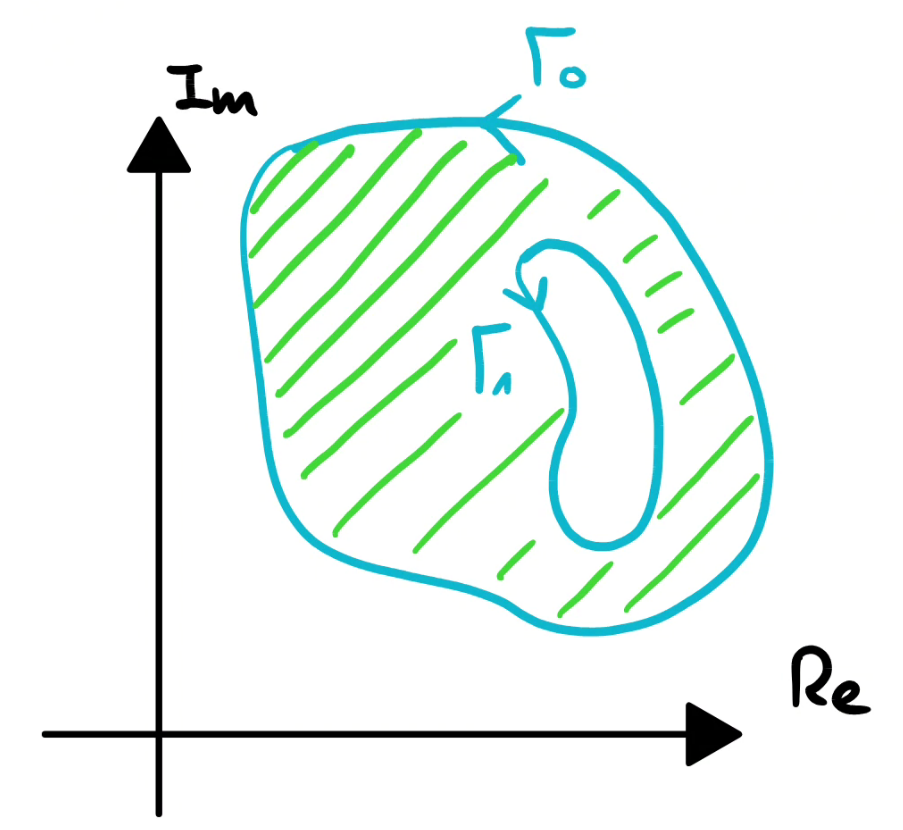
\includegraphics[width=0.4\linewidth]{Sketches/CauchysTheoremExtended}
	
	\label{fig:cauchystheoremextended}
\end{figure}


Let $\Gamma_0, \Gamma_1$ be two closed, simple, regular curves with the same orientation with $\Gamma_1\subseteq \operatorname{int} \Gamma_0$.
Let $f$ be a function with is holomorphic on $\operatorname{int} \Gamma_0\backslash \operatorname{int}\Gamma_1$.
Then: \footnote{A formal proof can be found in the lecture notes on Moodle.}
\begin{equation*}
	\boxed{\int_{\Gamma_0} f(z)\,dz = \int_{\Gamma_1} f(z)\,dz}
\end{equation*}

Furthermore, let $\Gamma_1,\Gamma_2$ be two curves with the same start- end endpoint and $f$ is holomorphic in the region contained between $\Gamma_1$ and $\Gamma_2$, then 
\begin{equation*}
	\int_{\Gamma_1} f(x)\,dx = \int_{\Gamma_2} f(x)\,dx
\end{equation*}

\subsection{Cauchy's Integral Formula}
\begin{figure}[H]
\begin{center}
	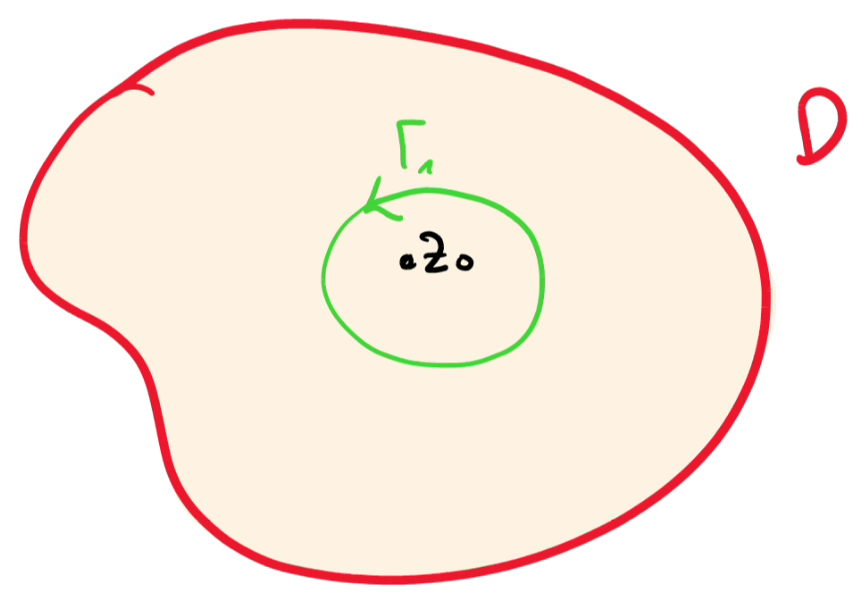
\includegraphics[width=0.3\linewidth]{Sketches/CauchyIntegralFormulas}
\end{center}
\end{figure}

Let $D \subseteq\mathbb C$ be an open set and $f:D\to \mathbb C$ be a holomorphic set. If $z_0\in D$, then:
\begin{equation*}
\boxed{f(z_0) = \frac 1{2\pi i} \int_\Gamma \frac{f(z)}{z-z_0}\,dz}
\end{equation*}
for any closed, simple curve $\Gamma$ inside $D$ which contains $z_0$ in its interior and is counter-clockwise oriented.

\subsubsection{Cauchy's Integral Formula Extended}

With the same assumptions as above,
\begin{equation*}
	f^{(n)}(z_0) = \frac{n!}{2\pi i}\int_{\Gamma} \frac{f(z)}{(z-z_0)^{(n + 1)}} \,dz
\end{equation*}

Through this formula we find the statement again, that holomorphic functions are infinitely differentiable.


\section{Laurent Series}

\subsection{Recall: Taylor Series for Real Numbers}
let $f:\mathbb R \to \mathbb R$ be a sufficiently regular function. For any $x_0\in \mathbb R$, the Taylor polynomial of degree $N$ is defined by:
\begin{equation*}
	T_{x_0}^Nf(x)=f(x_0)+ f'(x_0)(x-x_0)+\dots + \frac{f^{(n)}(x_0)}{N! }(x-x_0) = \sum_{n=0}^N \frac{f^{(n)}(x_0)}{n!}(x-x_0)^n
\end{equation*}
If $f\in C^{N+1}(\mathbb R)$, then $\forall x_0,x\in\mathbb R: \exists \theta \in]0,1[$ such that:
\begin{equation*}
	f(x)= T_{x_0}^N f(x)+ \frac{f^{(N+1)}(\theta x_0+(1-\theta)x)}{N+1!}(x-x_0)^{N+1}
\end{equation*}
In practice, $\theta$ is not known, but we can usually estimate the $N+1$ th derivative.

If $f$ has derivatives of all orders at $x_0$, then we may consider the Taylor series
\begin{equation*}
	\sum_{n=0}^\infty \frac{f^{(n)}(x_0)}{n!}(x-x_0)^n
\end{equation*}

Functions $f$ such that the Taylor series converges to $f$ in a neighbourhood of $x_0$ are called \textbf{analytic}, and therefore $C^\infty$. Not all $C^\infty$ functions are analytic.
\subsection{Taylor Series for Complex Functions: Regular Laurent Series}
Let $D\subseteq \mathbb C$ be an open set ant $z_0\in D$. Let $R> 0$ be such that the disc
\begin{equation*}
	B_R(z_0):=\{z:|z-z_0|<R\}
\end{equation*}
is contained in $D$. If $f:D\to \mathbb C$ is \textbf{holomorphic}, then \begin{equation*}
	f(z)=\sum_{n=0}^\infty \frac{f^{(n)}(z_0)}{n!}(z-z_0)^n
\end{equation*}
for all $z \in B_R(z_0)$.

The largest such $R > 0 $ is the \textbf{Radius of convergence.}

\paragraph{Remarks} Homomorphic functions $f$ are therefore analytic (around every $z_0$ in their domain, there exists a disk on which the Taylor series converges to $f$).

In practice, $R$ is the distance of $z_0$ from the "nearest" point where $f$ is not holomorphic or not defined.

We can connect the Taylor series to the Cauchy integral formula:
\begin{equation*}
	\sum_{n=0}^\infty \frac{f^{(n)(z_0)}}{n!}(z-z_0)^n = \sum_{n=0}^\infty c_n(z-z_0)^n
\end{equation*}
where
\begin{equation*}
	c_n = \frac{f^{(n)}(z_0)}{n!}= \frac 1{2\pi i} \int_\Gamma \frac{f(\zeta)}{\zeta - z_0}\,d\zeta
\end{equation*}

Note that this important result can be derived from the above:
\begin{equation*}
	\boxed{\sum_{n=0}^\infty z^n=\frac 1{1-z}} \qquad \forall |z|< 1
\end{equation*}


\subsection{Laurent Series}
Let $D\subseteq \mathbb C$ be an open set and $z_0\in D$. Suppose that:
\begin{equation*}
	f:D\backslash \{z_0\}\to\mathbb C
\end{equation*}
is holomorphic. Let $R > 0$ be such that $B_R(z_0)\subseteq D$. Then for all $z\in  B_R(z_0)\backslash\{z_0\}$:
\begin{equation}
	\boxed{f(z) = \sum_{-\infty}^\infty c_n(z-z_0)^n}
\end{equation}
where, for any simple, closed, counter-clockwise oriented curve $\Gamma$, such that the interior of $\Gamma$ is contained in $D$ and $z_0$ is in the interior of $\Gamma$, the coefficients $c_n$ are given by:
\begin{equation*}
	c_n = \frac 1{2\pi i} \int_ \Gamma\frac{f(\zeta)}{(\zeta - z_0)^{(n+1)}}\,d \zeta
\end{equation*}

\paragraph{Remarks} The Laurent series is like a Taylor series, but we now also include therms with polynomial singularities. As in the case of the Taylor series, the Laurent series is the \textbf{only} representation of $f$ as a power series. I.e. any other such series will have the same coefficients.

\subsubsection{Singular and Regular parts}
Any Laurent series splits into a \textbf{singular} and a \textbf{regular} part:
\begin{equation*}
	f(z) = \sum_{-\infty}^\infty c_n (z-z_0) ^n = \underbrace{\dots + \frac{c_{-2}}{(z-z_0)^2}+\frac{c_{-1}}{(z-z_0)}}_{\text{singular}} + \underbrace{c_0 + c_1(z-z_0) + \dots}_{\text{regular}}
\end{equation*}
The Taylor series is a Laurent series with no singular part.

